\documentclass[12pt, a4paper]{article}
\usepackage{../notesheets}


%%%%%%%%%%%%%%%%%%%%%%%%%%%%%%%%%%%%%%%%%%%%%%%%%%
\author{Math 1210}
\title{Related Rates Worksheet}
\date{}

\begin{document}
\maketitle
\thispagestyle{empty}
\subsection*{Some Useful Geometric Facts for Common Related Rates Problems}
\subsubsection*{Pythagorean Theorem}
\begin{center}
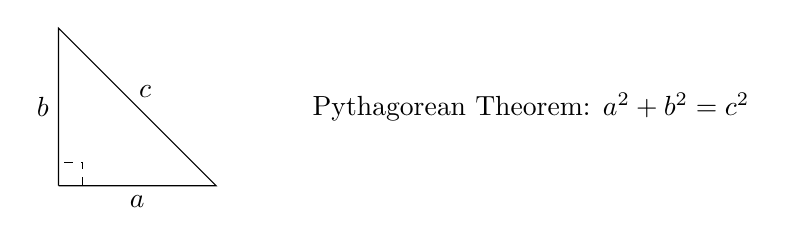
\begin{tikzpicture}
\draw (0,0)--(0,2)--(2,0)--(0,0);
\draw[dashed] (.3,0)--(.3,.3)--(0,.3);
\node[below] at (1,0) {$a$};
\node[left] at (0,1) {$b$};
\node at (1.1,1.2) {$c$};
\node at (6, 1) {Pythagorean Theorem: $a^2+b^2=c^2$};
\end{tikzpicture}

\end{center}
\subsubsection*{Area, Perimeter, Circumference Formulas}
\begin{center}
\vspace{1em}
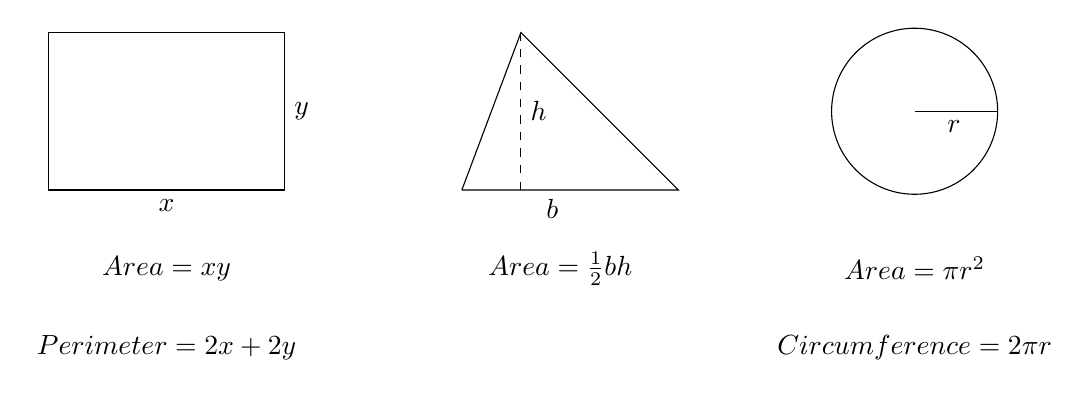
\begin{tikzpicture}
\draw (-4,0)--(-1,0)--(-1,2)--(-4,2)--(-4,0);
\node[below] at (-2.5,0) {$x$};
\node[right] at (-1,1) {$y$};
\node at (-2.5,-1) {$Area =xy$};
\node at (-2.5, -2) {$Perimeter =2x+2y$};

\draw (1.25,0)--(2,2)--(4,0)--(1.25,0);
\draw[dashed] (2,0)--(2,2);
\node[below] at (2.4,0) {$b$};
\node[right] at (2,1) {$h$};
\node at (2.5,-1) {$Area=\frac{1}{2}bh$};


\draw (7,1) circle(30pt);
\draw (7,1)--(8.05,1);
\node[below] at (7.5,1) {$r$};
\node at (7, -1) {$Area=\pi r^2$};
\node at (7,-2) {$Circumference =2\pi r$};
\end{tikzpicture}

\end{center}


\subsubsection*{Volume Formulas}

\begin{center}
\vspace{1em}
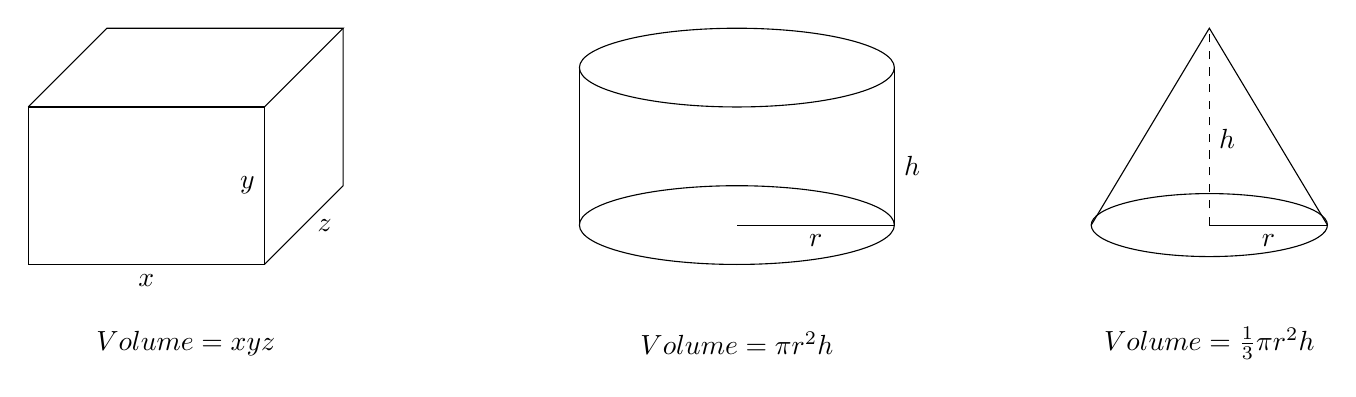
\begin{tikzpicture}
\draw (-4,0)--(-1,0)--(-1,2)--(-4,2)--(-4,0);
\draw (-4,2)--(-3,3)--(0,3)--(-1,2);
\draw (0,3)--(0,1)--(-1,0);
\node[below] at (-2.5,0) {$x$};
\node[left] at (-1,1) {$y$};
\node[right] at (-.45, .5) {$z$};
\node at (-2, -1) {$Volume = xyz$};

\draw (5,2.5) ellipse [x radius =2, y radius = .5];
\draw (5,.5) ellipse [x radius =2, y radius = .5];
\draw (3,2.5)--(3,.5);
\draw (7,2.5)--(7,.5);
\draw (7,.5)--(5,.5);
\node[below] at (6,.5) {$r$};
\node[right] at (7,1.25) {$h$};
\node at (5, -1) {$Volume = \pi r^2h$};

\draw (11,.5) ellipse [x radius =1.5, y radius = .4];
\draw (9.5, .5)--(11, 3)--(12.5,.5);
\draw[dashed] (11, .5)--(11,3);
\draw (11, .5)--(12.5,.5);
\node[below] at (11.75,.5) {$r$};
\node[right] at (11, 1.6) {$h$};
\node at (11, -1) {$Volume = \frac{1}{3}\pi r^2 h$};
\end{tikzpicture}

\end{center}

\subsection*{General Guidelines for Solving Related Rates Problems}
\begin{enumerate}
\item Assign a variable to each quantity. Draw a diagram if applicable.
\item Write down what we are trying to find as well as the given values of the variables and the given rates of change.
\item Write down any equation(s) that relate the variables.
\item Implicitly differentiate equation(s).
\item Solve for desired rate of change. Then state the final answer and remember to include units.
\end{enumerate}
\begin{ex}
  Car \(A\) is traveling west at \(50\) mi/h and car \(B\) is
  traveling north at \(60\) mi/h. Both are headed for the intersection
  of the two roads (denoted \(C\)). At what rate are the cars
  approaching each other
  when car \(A\) is \(0.3\) mi and car \(B\) is \(0.4\) mi from the
  intersection?
\end{ex}
\vspace{-2in}
\begin{enumerate}
\item \includegraphics[scale=0.5]{images/cars-at-intersection}

\item   \(\frac{dx}{dt} = \) \hspace{2in} What are we trying to find?
  \\ \\
   \(\frac{dy}{dt} = \)
\item What is the relationship
  between \(x,y,\) and \(z\)?
  \vspace{1in}
\item Implicitly differentiate the relationship you found above.
  \vspace{1in}
\item Solve the equation above for \(\frac{dz}{dt}\). Your answer will
  be in terms of \(x,y,z,\frac{dx}{dt},\) and
  \(\frac{dy}{dt}\). Finally, plug in the desired values \(x=0.3\) mi,
  \(y = 0.4\) mi, the value of \(z\) (from the
  relationship in part (c)), and what you found for \(\frac{dx}{dt}\) and
  \(\frac{dy}{dt}\) in part (a).
\end{enumerate} \vspace{1in}
\begin{ex}
  Now, do WebAssign 3.6 some of questions \(7\)--\(12\) for practice.
\end{ex}
\vspace{-2.5in}
\begin{ex}
  \textbf{Write out your solution on a separate piece of paper using the
  structure of the solution above as a template.} Suppose that water
is flowing out of a hole at the bottom of a cone into a cylinder
located below the bottom of the cone. Suppose that the height of the
water in the cone is decreasing at a constant rate of $2\ cm/sec$. The
cone has radius $10\ cm$ and height $20\ cm$. The cylinder has radius
$30\ cm$ and height $70\ cm$. For simplicity, assume that as soon as
water leaves the hole of the cone it instantaneously goes into the
cylinder. In other words, it takes 0 time for the water to fall from
the hole into the cylinder. What is the rate of change of the height
of the water in the cylinder when the height of the water in the cone
is $4\ cm$? \textbf{(Hint: Use
  Similar Triangles)}
\end{ex}
3 (a) \\
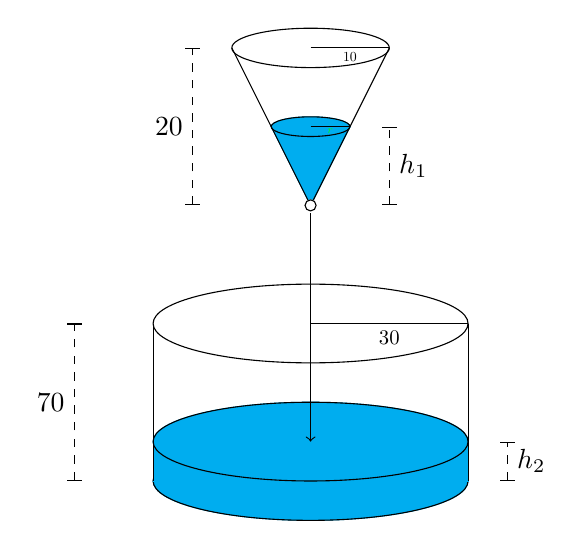
\begin{tikzpicture}
\filldraw[cyan] (5,.5) ellipse [x radius =2, y radius = .5];
\draw (5,.5) ellipse [x radius =2, y radius = .5];
\filldraw[cyan](3,.5)  rectangle (7,1);
\filldraw[cyan] (5,1) ellipse [x radius =2, y radius = .5];
\draw (5,1) ellipse [x radius =2, y radius = .5];
\filldraw[cyan] (5,4)--(4.5,5)--(5.5,5)--(5,4);
\filldraw[cyan] (5,5) ellipse [x radius =.5, y radius = .125];
\draw (5,5) ellipse [x radius =.5, y radius = .125];
\draw (5,6) ellipse [x radius =1, y radius = .25];
\draw (4,6)--(5,4)--(6,6);
\draw (5,2.5) ellipse [x radius =2, y radius = .5];
\filldraw[white] (5,4) circle(2pt);
\draw (5,4) circle(2pt);
\draw[->] (5,3.9)--(5,1);
\draw[dashed,|-|] (3.5,4)--(3.5,6);
\node[left] at (3.5,5) {$20$};
\draw[dashed,|-|] (6,4)--(6,5);
\node[right] at (6,4.5) {$h_{1}$};
\draw (5,6)--(6,6);
\node[below, scale = .5] at (5.5, 6) {$10$};
\draw (5, 5)--(5.5,5);
\node[green, scale = .4] at (5.25, 4.94) {$r$};
\draw[dashed,|-|] (2,.5)--(2,2.5);
\node[left] at (2,1.5) {$70$};
\draw[dashed,|-|] (7.5,.5)--(7.5,1);
\node[right] at (7.5,.75) {$h_{2}$};
\draw (5,2.5)--(7,2.5);
\node[below, scale =.75] at (6,2.5) {$30$};

\draw (3,2.5)--(3,.5);
\draw (7,2.5)--(7,.5);
\end{tikzpicture}
\end{document}
